\documentclass[11pt,letterpaper]{article}
\usepackage{times}
\usepackage[onehalfspacing]{setspace}
\usepackage{natbib}\bibpunct{(}{)}{,}{}{}{,}
\usepackage{amsmath,amsfonts,amsthm}
\usepackage{comment}
\usepackage{tabularx}
\usepackage{multirow}
\usepackage{booktabs}
\usepackage{subcaption}
\usepackage{graphicx}
\usepackage[colorlinks,linkcolor=blue,citecolor=black,urlcolor=black]{hyperref}
\usepackage[title,titletoc]{appendix}
\usepackage{enumitem}
\usepackage{subcaption}  % For subfigures
\usepackage{lscape}      % For landscape orientation if needed
\usepackage[noabbrev,capitalize]{cleveref}
\usepackage{tikz}
\usetikzlibrary{shapes.geometric}
\usepackage{pgfplots}
\usetikzlibrary{patterns, pgfplots.fillbetween}
\usepackage{graphicx}
\usepackage{mathpazo}

% commands
\newtheorem{definition}{Definition}
\newtheorem{proposition}{Proposition}
\newtheorem{lemma}{Lemma}
\newcommand{\figpath}{fig/}
\newcommand{\tablepath}{table/}
\newcommand{\rmdi}{\mathrm{d}}

% table and figure formatting
%\input{formats}

% page size
\setlength{\textwidth}{\paperwidth}
\addtolength{\textwidth}{-1.7in}
\setlength{\oddsidemargin}{.85in}
\addtolength{\oddsidemargin}{-.85in}
\setlength{\evensidemargin}{\oddsidemargin}
\setlength{\headheight}{0pt}
\setlength{\headsep}{0pt}
\setlength{\textheight}{\paperheight}
\addtolength{\textheight}{-\headheight}
\addtolength{\textheight}{-\headsep}
\addtolength{\textheight}{-\footskip}
\addtolength{\textheight}{-1.75in}
\setlength{\topmargin}{1in}
\addtolength{\topmargin}{-1in}

\begin{document}

\title{\textbf{Hecksher-Ohlin Model and the Three Big Theorems of International Trade}}
\author{\large%
\setcounter{footnote}{0}%
Carlos G\'{o}es \\[-3pt] \textit{\small IFC, World Bank Group}
}
\maketitle

\paragraph{Production} Consider a world with 2 countries $i \in \{ H, F\}$ and two industries: cloth $C$ and tech $T$. In country $i$, there are $\bar{L}_i$ units of labor (worker-hours) available, which we call the labor endowment. There is also a fixed stock of capital denoted by $\bar{K}_i$. In country $i$, firms producing good $g \in \{ C, T\}$ have a Cobb-Douglas technologies satisfying:

\begin{equation*}
 Y_{i,C} = K_{i,C}^{\beta_C} L_{i,C}^{1-\beta_C}, \qquad  Y_{i,T} = K_{i,T}^{\beta_T} L_{i,T}^{1-\beta_T}
\end{equation*}

Unlike in the specific factors model, here both models use both factors -- i.e., there is no \textit{specific} factor. However, here we assume that the technology is different in each sector (albeit common across countries). Specifically, the Cobb-Douglas parameters $\{\beta_C,\beta_T\}$. Specifically, we assume that the returns to capital are higher in the tech sector relative to cloth, i.e.: $\beta_T > \beta_C$.

Both labor and capital are common factors which are freely mobile across sectors.This means that, after some change in relative prices (or to some fundamentals that alter the marginal product of any of the factors), labor and capital will to move across sectors to optimize the level of production and consumption. Labor and capital allocations must satisfy:

\begin{equation*}
    L_{i,T} + L_{i,C} \le \bar{L}_i, \qquad K_{i,T} + K_{i,C} \le \bar{K}_i
\end{equation*}

\noindent i.e., the sum of the labor and capital used in agriculture and manufacturing, respectively, cannot be larger than the total labor endowment in the country. Firms take factor prices as given and maximize profits under perfect competition:
        \begin{eqnarray*}\label{eq: production}
            &\max_{L_{i,C}, K_{i,C}}& P_{C} \times K_{i}^{\beta_C} L_{i,C}^{1-\beta_C} - w_i L_{i,C} - r_{i} K_{i,C} \\
            &\max_{L_{i,T}, K_{i,T}}& P_{T} \times K_{i}^{\beta_T} L_{i,T}^{1-\beta_T} - w_i L_{i,T} - r_{i} K_{i,T} 
        \end{eqnarray*}

This is a simple unconstrained maximization problem that you can solve by taking a derivative of the objective function with respect to each choice variable and setting it equal to zero. Note that, since labor and capital are mobile factors, there will be common prices for wage $w_i$ and rents $r_i$. 

The optimal choices satisfy the marginal product of each factor (converted to dollars) being equal to their factor prices (why?):

\begin{eqnarray}
    P_{C} \times (1-\beta_C) \times \left( \frac{K_{i,C}}{L_{i,C}} \right)^{\beta_C} = P_C \times MPL_{i,C} &=& w_i     \\
    P_{C} \times  \beta_C \times \left( \frac{L_{i,C}}{K_{i,C}} \right)^{1-\beta_C} = P_C \times MPK_{i,C} &=& r_{i}   \\
    P_{T} \times (1-\beta_T) \times \left( \frac{K_{i,T}}{L_{i,T}} \right)^{\beta_T} =  P_T \times MPL_{i,T} &=& w_i \\ 
     P_{T}  \times \beta_T \times \left( \frac{L_{i,T}}{K_{i,T}} \right)^{1-\beta_T}    = P_T \times MPK_{i,T} &=& r_{i} 
\end{eqnarray}

The wage rage $w_i$ will be such that $L_{i,T} + L_{i,C} = \bar{L}_i$, as in the specific factors model. Since capital is also mobile, the wage rage $r_i$ will similarly be such that $K_{i,T} + K_{i,C} = \bar{K}_i$. Dividing the two first equations and two last equations, respectively, we find that:

\begin{eqnarray}\label{eq: capital-labor}
    \frac{K_{i,C}}{L_{i,C}} = \frac{\beta_C}{1-\beta_C} \times \frac{w_i}{r_i}, \qquad \frac{K_{i,T}}{L_{i,T}} = \frac{\beta_T}{1-\beta_T} \times \frac{w_i}{r_i} 
\end{eqnarray}

At the optimal choices, the capital-to-labor ratio in each industry is inversely proportional to their factor prices, scaled by factor intensities $\beta_g$.  What is the intuition? The ratio of factor prices $w_i/r_i$ will tell us how firms allocate how many machines they buy for each worker they hire. If the price of labor is expensive relative to the price of machines ($w_i/r_i$ is high), then firms will substitute labor for capital. The intensity of this relationship is controlled by the parameters $\{\beta_T, \beta_C\}$. Since $\beta_T > \beta_C$, then $ \frac{K_{i,T}}{L_{i,T}} > \frac{K_{i,C}}{L_{i,C}} $ at the optimal choices for \textbf{any} equilibrium factor prices.

We can also show that there is a relationship between factor prices $w_i / r_i$ and goods prices $P_C / P_T$. First, combining equations (1) and (3), note that:

\begin{eqnarray}
    \frac{P_C}{P_T} = \frac{MPL_{i,T}}{MPL_{i,C}} \iff 
    \frac{P_C}{P_T} = \frac{(1-\beta_T) \times \left( \frac{K_{i,T}}{L_{i,T}} \right)^{\beta_T}}{ (1-\beta_C) \times \left( \frac{K_{i,C}}{L_{i,C}} \right)^{\beta_C}}  
\end{eqnarray}

Here the intuition is that marginal revenue must equalize across sectors when using the same factor. Whenever the price of cloth is high relative to tech ($P_C/P_T$ is high) then the cloth sector will use proportionately more labor than the tech sector. If $\frac{MPL_{i,T}}{MPL_{i,C}}$ is high, this means that the marginal product of labor is proportionately high in the tech sector relative to the cloth sector. Since we know $MPL$ is decreasing in labor, this means that there is much proportionately labor in $T$ relative to $C$ (use the functional forms if you are confused).

\paragraph{Stolper-Samuelson Theorem (weak form)} For now we have seen that we can map from factor prices to the capital-to-labor ratio \textit{and} from relative marginal products to goods prices. Combining these two results and replacing from equation \eqref{eq: capital-labor}:

\begin{eqnarray}\label{eq: goods-factor-prices}
    \frac{P_C}{P_T} = \frac{(1-\beta_T) \times \left( \frac{\beta_T}{1-\beta_T} \times \frac{w_i}{r_i}  \right)^{\beta_T}}{ (1-\beta_C) \times \left( \frac{\beta_C}{1-\beta_C} \times \frac{w_i}{r_i} \right)^{\beta_C}} \iff \frac{P_C}{P_T} = \frac{(1-\beta_T)^{1-\beta_T} \beta_T^{\beta_T}}{ (1-\beta_C)^{1-\beta_C} \beta_C^{\beta_C} } \times \left(  \frac{w_i}{r_i} \right)^{\beta_T - \beta_C}
\end{eqnarray} 

Since $\beta_T > \beta_C$, goods prices $P_C/P_T$ is increasing in factor prices $w_i/r_i$. This show that if the \textit{relative price of one good increases}, the \textit{relative income of the factor that is relatively intensively used in the good’s production increases}. Above, we see that if the price of cloth relative to tech increases, since cloth is labor intensive relative to cloth (which is capital intensive), then the price of labor relative to capital must increase. This is the main result of the \textbf{Stolper-Samuelson theorem} (in its weak form). We will go deeper into the theorem later. For now, let's focus on the intuition.

\begin{figure}[htp]
    \centering
    \begin{tikzpicture}
    \begin{axis}[
        axis lines=middle,
        xmin=-1.1, xmax=1.1,
        ymin=0, ymax=1.1,
    %    xlabel={\small Output of manufactures / Labor in manufactures},
    %    ylabel={\small Output of food / Labor in food},
        xtick=\empty,
        ytick=\empty,
        width=15cm,
        height=8cm,
        axis line style={<->},
        clip=false,
        enlargelimits=false,
        domain=0.0:1,
        samples=200
    ]
    
    \pgfmathsetmacro{\a}{0.5}       % curvature parameter
    \pgfmathsetmacro{\betac}{1/3}       % curvature parameter
    \pgfmathsetmacro{\betat}{2/3}       % curvature parameter
    \pgfmathsetmacro{\c}{(\betac)^(\betac)*(1-\betac)^(1-\betac)}        \pgfmathsetmacro{\t}{(\betat)^(\betat)*(1-\betat)^(1-\betat)}        \pgfmathsetmacro{\rw}{1/4}
    \pgfmathsetmacro{\prw}{-(\c / \t * (\rw)^(\betat- \betac)}
    \pgfmathsetmacro{\rww}{1/2}
    \pgfmathsetmacro{\prww}{-(\c / \t * (\rww)^(\betat- \betac)}
    % curvature parameter
% curvature parameter
    
    % NW: Production function for food (plot in 2nd quadrant)
    \addplot[brown] ({x}, {(1-\betat)/\betat * x});
    \addplot[red, domain=0:0.5] ({x}, {(1-\betac)/\betac * x});
    \addplot[blue] ({-x}, {\t / \c * (x)^(1/(\betat - \betac))});
    \node[anchor=east] at (axis cs:-1.1,0) {  $P_C/P_T$};
    \node[anchor=west] at (axis cs:1.1,0) {  $K_{i,g}/L_{i,g}$};
    \node[anchor=south] at (axis cs:0,1.1) { $w_i/r_i$};

    %old eqm
    \addplot[dashed, gray] coordinates {(\prw, \rw) (\betat / (1-\betat) * \rw, \rw)};
    \addplot[dashed, gray] coordinates {(\prw, \rw) (\prw , 0)};
    \node[anchor=north] at (axis cs:\prw , 0) {$\frac{P_C}{P_T}$};
    \addplot[mark=*, black, mark size=1.5pt] coordinates {(\prw,\rw)};
    \addplot[mark=*, black, mark size=1.5pt] coordinates {(0,\rw)};
    \node[anchor=south east] at (axis cs:0,\rw) {$\frac{w_i}{r_i}$};
    \addplot[mark=*, black, mark size=1.5pt] coordinates {(\betac / (1-\betac) * \rw,\rw)};
    \addplot[dashed, gray] coordinates {(\betac / (1-\betac) * \rw, \rw) (\betac / (1-\betac) * \rw , 0)};
    \node[anchor=north] at (axis cs:{\betac / (1-\betac) * \rw} , 0) {$\frac{K_C}{L_C}$};
    \addplot[mark=*, black, mark size=1.5pt] coordinates {(\betat / (1-\betat) * \rw,\rw)};
    \addplot[dashed, gray] coordinates {(\betat / (1-\betat) * \rw, \rw) (\betat / (1-\betat) * \rw , 0)};
    \node[anchor=north] at (axis cs:{\betat / (1-\betat) * \rw} , 0) {$\frac{K_T}{L_T}$};

    %new eqm
    \addplot[dashed, gray] coordinates {(\prww, \rww) (\betat / (1-\betat) * \rww, \rww)};
    \addplot[dashed, gray] coordinates {(\prww, \rww) (\prww , 0)};
    \node[anchor=north] at (axis cs:\prww , 0) {$\left( \frac{P_C}{P_T} \right)'$};
    \addplot[mark=*, black, mark size=1.5pt] coordinates {(\prww,\rww)};
    \addplot[mark=*, black, mark size=1.5pt] coordinates {(0,\rww)};
    \node[anchor=south east] at (axis cs:0,\rww) {$\left( \frac{w_i}{r_i} \right)'$};
    \addplot[mark=*, black, mark size=1.5pt] coordinates {(\betac / (1-\betac) * \rww,\rww)};
    \addplot[dashed, gray] coordinates {(\betac / (1-\betac) * \rww, \rww) (\betac / (1-\betac) * \rww , 0)};
    \node[anchor=north] at (axis cs:{\betac / (1-\betac) * \rww} , 0) {$\frac{K_C'}{L_C'}$};
    \addplot[mark=*, black, mark size=1.5pt] coordinates {(\betat / (1-\betat) * \rww,\rww)};
    \addplot[dashed, gray] coordinates {(\betat / (1-\betat) * \rww, \rww) (\betat / (1-\betat) * \rww , 0) };
    \node[anchor=north] at (axis cs:{\betat / (1-\betat) * \rww} , 0) {$\frac{K_T'}{L_T'}$};

    % slope
    \pgfmathsetmacro{\rws}{3/4}
    \addplot[dashed, gray] coordinates {(\betac / (1-\betac) * \rws, \rws) (\betac / (1-\betac) * (\rws + .2), \rws) };
    \node[anchor=north west] at (axis cs:{\betac / (1-\betac) * \rws}, \rws) {$1$};
    \addplot[dashed, gray] coordinates {(\betac / (1-\betac) * (\rws + .2), \rws) (\betac / (1-\betac) * (\rws + .2), \rws + .2)  };
    \node[anchor=south west] at (axis cs:{\betac / (1-\betac) * (\rws + .2)}, \rws) {$\frac{1-\beta_C}{\beta_C}$};

    \pgfmathsetmacro{\rwss}{0.3}
    \addplot[dashed, gray] coordinates {(\betat / (1-\betat) * \rwss, \rwss) (\betat / (1-\betat) * (\rwss + .065), \rwss) };
    \node[anchor=north west] at (axis cs:{\betat / (1-\betat) * \rwss}, \rwss) {$1$};
    \addplot[dashed, gray] coordinates {(\betat / (1-\betat) * (\rwss + .065), \rwss) (\betat / (1-\betat) * (\rwss + .065), \rwss + .065)  };
    \node[anchor=south west] at (axis cs:{\betat / (1-\betat) * (\rwss + .065)}, \rwss-.05) {$\frac{1-\beta_T}{\beta_T}$};
     \end{axis}
    
    \end{tikzpicture}
    \caption{xx}
    \label{fig: signature}

\end{figure}

We summarize these relationships between goods prices, factor prices, and capital-to-labor ratios in Figure \ref{fig: signature}. Suppose that the initial relative prices are $P_C /P_T$. This pins down the relative factor prices $w_i/r_i$, which in turn pins down the capital-to-labor ratios. Note that, as expected, $K_T/L_T > K_C/L_C$. Now suppose that the relative price of cloth increases to $(P_C /P_T)' > P_C /P_T$. Since the cloth sector is labor intensive, the relative factor price of labor increases to $(w_i/r_i)'>w_i/r_i$. Since labor is now relatively more expensive, both sectors start using more capital relative to labor: $K'_C/L'_C > K_C/L_C$ and $K'_T/L'_T > K_T/L_T$

\paragraph{Stolper-Samuelson Theorem (strong form)} For now we have shown that when \textit{relative price of one good increases}, the \textit{relative income of the factor that is relatively intensively used in the good’s production increases}. But the theorem goes beyond that. In its strong form, it states that \textit{if the relative price of one good increases, the \textbf{real income} of the factor that is used intensively in production of the good will increase,
while the other factor’s real income falls}.

In other words, the prediction is what we call a \textit{magnification effect}. Let $\hat{x} = (x'-x)/x$ be the percent change in variable $x$. The magnification effect prediction is that:

\begin{equation*}
    \hat{w}_i > \hat{P}_C > \hat{P}_T > \hat{r}_i
\end{equation*}

\noindent in other words, the change in the relative factors prices $w_i/r_i$ will be \textbf{larger} than the change in relative goods prices $P_C/P_T$. Using the specific functional forms that we use in this course, it is easy to see from equation \eqref{eq: goods-factor-prices} and Figure \ref{fig: signature} that relative goods prices are a concave function of relative factor prices:

\begin{equation*}
    \frac{P_C}{P_T} = \text{constant} \times \left( \frac{w_i}{r_i} \right)^{\beta_T - \beta_C}, \qquad \text{for } 0<\beta_T - \beta_C<1
\end{equation*}

\noindent so $P_C/P_T$ grows less than proportional to the increase in $w_i/r_i$. Jones (1965) provides a more general proof of the strong form of the theorem, which is beyond the scope of this course.

\paragraph{Edgeworth Box} How can both sectors raise the relative use of capital? The cloth sector expands while tech sector contracts. Cloth producers hire more workers and rent more machines to expand production, but they rent proportionally more machines than workers (which is not hard, since they are labor-intensive). Tech producers fire workers and cancel contracts for machines to contract production, but they fire proportionately more workers than machines (which is not hard, since they are capital-intensive).

One way to see this algebraically. Using the resource constraint for capital, we can show:

\begin{equation}\label{eq: constrants-ratio}
    \frac{\bar{K}_i}{\bar{L}_i} = \frac{K_{i,C}}{\bar{L}_i} + \frac{K_{i,T}}{\bar{L}_i} \iff \frac{\bar{K}_i}{\bar{L}_i} = \frac{K_{i,C}}{L_{i,C}} \frac{L_{i,C}}{\bar{L}_i} + \frac{K_{i,T}}{L_{i,T}} \frac{L_{i,T}}{\bar{L}_i}  \iff \frac{\bar{K}_i}{\bar{L}_i} = \frac{K_{i,C}}{L_{i,C}} \times \ell_{i,C} + \frac{K_{i,T}}{L_{i,T}} \times (1-\ell_{i,C})
\end{equation}

Above, since $\frac{\bar{K}_i}{\bar{L}_i}$ is fixed and $\frac{K_{i,T}}{L_{i,T}} > \frac{K_{i,C}}{L_{i,C}}$, if both sectors increase their capital-to-labor ratio, then $\ell_{i,C}$ must increase to put a higher weight in the least capital intensive industry. Another (more intuitive) way to visualize these changes is with a diagram. We illustrate these changes in Figure \ref{fig: factor-mkt-eqm-trade}. In the Figure, there are two overlapping diagrams. The standard, with an origin in the southwest corner, shows every possible choice for $\{L_{i,C},K_{i,C}\}$, up to the endowments $\{\bar{L}_{i},\bar{K}_{i}\}$. An inverted axis, with origin in the Northeast corner, shows every possible choice for $\{L_{i,T},K_{i,T}\}$. This figure is called an \textit{Edgeworth Box} and it is used in different parts of economics.

\begin{figure}
    \centering
    \begin{tikzpicture}
    
    % Setup axis
    \begin{axis}[
        axis lines=middle,
        xtick=\empty,
        ytick=\empty,
        xmin=0, xmax=1,
        ymin=0, ymax=1,
        samples=300,
        axis line style={->},
        width=16cm,
        height=8cm,
        domain=0:1,
        clip=false,
    ]
    \pgfmathsetmacro{\betat}{2/3}
    \pgfmathsetmacro{\betac}{1/3}
    \pgfmathsetmacro{\bc}{(1-\betac)/\betac}
    \pgfmathsetmacro{\bt}{(1-\betat)/\betat}

    
    \addplot[->] coordinates {(1,1) (0,1)};
    \addplot[->] coordinates {(1,1) (1,0)};
    
    \node[anchor=north] at (axis cs:1, 0) {$\bar{L}_{i}$};
    \node[anchor=east] at (axis cs:0, 1) {$\bar{K}_{i}$};
    \node[anchor=west] at (axis cs:1, 0) {$\bar{K}_{i}$};
    \node[anchor=south] at (axis cs:0, 1) {$\bar{L}_{i}$};

    \node[anchor=north] at (axis cs:0, 0) {$0$};
    \node[anchor=east] at (axis cs:0, 0) {$0$};
    \node[anchor=west] at (axis cs:1, 1) {$0$};
    \node[anchor=south] at (axis cs:1, 1) {$0$};


    % contract curve comes from equating the two K/L equations and using the two resource constraints to sovle for K as a function of L
    \addplot[gray, thick, domain=0:1] ({x}, {\bt * x / ( \bc * (1-x) + \bt * x )});

    \foreach \x [count=\i from 1] in {0.25, 0.75}
    {
        \addplot[red!50, thick,->>] coordinates {(0,0) (\x,{\bt * \x / ( \bc * (1-\x) + \bt * \x )})};
        \addplot[mark=*, black, mark size=1.5pt] coordinates {(\x,{\bt * \x / ( \bc * (1-\x) + \bt * \x )})};
        \addplot[blue!50, thick, ->>] coordinates {(1,1) (\x,{\bt * \x / ( \bc * (1-\x) + \bt * \x )})};
        \addplot[dashed, gray] coordinates {(0,{\bt * \x / ( \bc * (1-\x) + \bt * \x )}) (\x,{\bt * \x / ( \bc * (1-\x) + \bt * \x )})  };
        \addplot[dashed, gray] coordinates {(1,{\bt * \x / ( \bc * (1-\x) + \bt * \x )}) (\x,{\bt * \x / ( \bc * (1-\x) + \bt * \x )})  };
        \addplot[dashed, gray] coordinates {(\x,{\bt * \x / ( \bc * (1-\x) + \bt * \x )}) (\x,0)  };
        \addplot[dashed, gray] coordinates {(\x,{\bt * \x / ( \bc * (1-\x) + \bt * \x )}) (\x,1)  };
    }

    \node[anchor=north] at (axis cs:(0.25,{\bt * 0.25 / ( \bc * (1-0.25) + \bt * 0.25 )}) {$1$};
    \node[anchor=east] at (axis cs:(0,{\bt * 0.25 / ( \bc * (1-0.25) + \bt * 0.25 )}) {$K_{i,C}$};
    \node[anchor=north] at (axis cs:0.25,0) {$L_{i,C}$};
    \node[anchor=west] at (axis cs:(1,{\bt * 0.25 / ( \bc * (1-0.25) + \bt * 0.25 )}) {$K_{i,T}$};
    \node[anchor=south] at (axis cs:0.25,1) {$L_{i,T}$};


    \node[anchor=north] at (axis cs:(0.75,{\bt * 0.75 / ( \bc * (1-0.75) + \bt * 0.75 )}) {$2$};
    \node[anchor=east] at (axis cs:(0,{\bt * 0.75 / ( \bc * (1-0.75) + \bt * 0.75 )}) {$K_{i,C}'$};
    \node[anchor=north] at (axis cs:0.75,0) {$L_{i,C}'$};
    \node[anchor=west] at (axis cs:(1,{\bt * 0.75 / ( \bc * (1-0.75) + \bt * 0.75 )}) {$K_{i,T}'$};
    \node[anchor=south] at (axis cs:0.75,1) {$L_{i,T}'$};


    % Bottom left and right axis labels
    %\node[below] at (axis cs:-0.5,-0.02) {\scriptsize $L_M$};
    %\node[below] at (axis cs:0.5,-0.02) {\scriptsize $L - L_M~(= L_F)$};
    
    \end{axis}
    
    \end{tikzpicture}
    \caption{Factor Markets Equilibrium}
    \label{fig: factor-mkt-eqm-trade}
\end{figure}

The initial equilibrium (before the increase in prices) is point $1$ in the diagram. It shows a smaller cloth sector relative to tech. The slopes of the red and blue arrows denote the capital-to-labor ratios (remember: for the slope we divide the rise -- capital input -- over run -- labor input). From this we can see that the the cloth sector uses very capital relative to labor (the slope is very flat) while the tech sector is, as expected, relatively more capital intensive (the slope is steeper). Once relative prices $P_C / P_T$ increase, the equilibrium moves to point $2$. The cloth sector expands and the tech sector contracts, so the red arrow becomes longer and the blue arrow becomes shorter. Both arrows become steeper, reflecting the fact that both industries are more capital intensive after the change in prices. The gray curve connecting the two origin points is called the \textit{contract curve}. It denotes every possible equilibrium with choices of $\{L_{i,C},K_{i,C},L_{i,T},K_{i,T}\}$ (it is convex relative to the Southwest origin because the tech sector is capital intensive relative to the cloth sector!).




\paragraph{Rybczynski Theorem} The Rybczynski Theorem is another major result of international trade. It states that, with both goods produced and fixed relative goods prices, an increase in the endowment of the factor used intensively in a given sector raises the output of that sector and decreases the output of the other sector. We will cover it graphically and algebraically here.

First, note that, since relative goods prices are assumed to be fixed, both $P_C/P_T$ and $w_i / r_i$ (because the latter are pinned down by the former). Second, since capital-to-labor ratios are pinned down by $w_i / r_i$, $K_g / L_g$ are also unchanged in both sectors. Let's first explore this issue graphically.
\begin{figure}[htbp!]
\centering
    \begin{tikzpicture}
    \pgfmathsetmacro{\alpha}{0.5}
    \pgfmathsetmacro{\betat}{5/6}
    \pgfmathsetmacro{\betac}{1/6}

    \pgfmathsetmacro{\L}{1}
    \pgfmathsetmacro{\K}{1}

    \pgfmathsetmacro{\Lc}{\alpha*(1-\betac) / ((1-\alpha)* (1-\betat) + \alpha*(1-\betac)) * \L}
    \pgfmathsetmacro{\Kc}{\alpha*(\betac) / ((1-\alpha)* (\betat) + \alpha*(\betac)) * \K}
    \pgfmathsetmacro{\Lt}{\L - \Lc}
    \pgfmathsetmacro{\Kt}{\K - \Kc}

    \pgfmathsetmacro{\wr}{ \K / \L * (\alpha*(1-\betac) + (1-\alpha)*(1-\betat))/(\alpha * \betac + (1-\alpha)*\betat)  }

    \pgfmathsetmacro{\P}{ ( ((1-\betat)^(1-\betat) * \betat^(\betat)) / ((1-\betac)^(1-\betac) * \betac^(\betac)) ) * (\wr)^(\betat-\betac)  }
    
    \pgfmathsetmacro{\Yc}{ \Kc^(\betac) * \Lc^(1-\betac) }
    \pgfmathsetmacro{\Yt}{ \Kt^(\betat) * \Lt^(1-\betat) }

    \pgfmathsetmacro{\U}{(\Yc^(\alpha))*(\Yt^(1 - \alpha))}
    \pgfmathsetmacro{\expo}{(1 - \alpha)/\alpha}
    \pgfmathsetmacro{\A}{\U^(1/\alpha)}
    
    \pgfmathsetmacro{\Kk}{1.25}

    \pgfmathsetmacro{\Lck}{\alpha*(1-\betac) / ((1-\alpha)* (1-\betat) + \alpha*(1-\betac)) * \L}
    \pgfmathsetmacro{\Kck}{\alpha*(\betac) / ((1-\alpha)* (\betat) + \alpha*(\betac)) * \Kk}
    \pgfmathsetmacro{\Ltk}{\L - \Lck}
    \pgfmathsetmacro{\Ktk}{\Kk - \Kck}

    \pgfmathsetmacro{\wrk}{ \wr  }

    \pgfmathsetmacro{\Pk}{ ( ((1-\betat)^(1-\betat) * \betat^(\betat)) / ((1-\betac)^(1-\betac) * \betac^(\betac)) ) * (\wrk)^(\betat-\betac)  }
    
    \pgfmathsetmacro{\Yck}{ \Kck^(\betac) * \Lck^(1-\betac) }
    \pgfmathsetmacro{\Ytk}{ \Ktk^(\betat) * \Ltk^(1-\betat) }


    \pgfmathsetmacro{\Uk}{(\Yck^(\alpha))*(\Ytk^(1 - \alpha))}
    
    % Compute prefactor for indifference curve: Qc = A * Qr^(- (1 - alpha)/alpha)
    \pgfmathsetmacro{\Ak}{\Uk^(1/\alpha)}
    
    \centering
    \begin{axis}[
        ylabel={Quantity of tech, $\textcolor{blue}{Y_{i,T}}$},
        xlabel={Quantity of cloth, $\textcolor{blue}{Y_{i,C}}$},
        ymin=0, ymax=\L+.5,
        xmin=0, xmax=\L+.5,
        yticklabel=\empty,
        xticklabel=\empty,
        axis lines=left,
        enlargelimits=false,
        clip=false,
        axis on top,
        scaled x ticks=false,
        width=9cm, height=7cm,
        title style={font=\bfseries}
    ]
    
    % PPF: Q_C = (L/a_C) - (a_R/a_C) * Q_R
    \addplot[blue, thick, domain=0:1] ({ \Kc^(\betac) * (\L-x)^(1-\betac)}, { \Kt^(\betat) * (x)^(1-\betat)});
    \pgfmathsetmacro{\c}{ \Yt + \P * \Yc }
    \addplot[thick, brown, domain=0.2:1.2] { \c - \P*x};
    

    % Equilibrium point
    \addplot[only marks, mark=*, color=black, mark size=2pt] coordinates {(\Yc, \Yt)};
    \addplot[dashed, gray] coordinates {(0,0) (\Yc, \Yt) };
    \node at (axis cs:\Yc - .15,\Yt - 0.1) {\scriptsize $(Y_{i,C},Y_{i,T})$};
        
    \addplot[blue, thick, domain=0:1] ({ \Kck^(\betac) * (\L-x)^(1-\betac)}, { \Ktk^(\betat) * (x)^(1-\betat)});
    \pgfmathsetmacro{\ck}{ \Ytk + \Pk * \Yck }
    \addplot[thick, brown, domain=0.2:1.2] { \ck - \Pk*x};
    
    
    % Equilibrium point
    \addplot[only marks, mark=*, color=black, mark size=2pt] coordinates {(\Yck, \Ytk)};
    \addplot[dashed, gray] coordinates {(0,0) (\Yck, \Ytk) };
    \node at (axis cs:\Yck + .15,\Ytk+ 0.1) {\scriptsize $(Y'_{i,C},Y'_{i,T})$};

    
    \end{axis}

\end{tikzpicture}

\caption{Expansion of Capital Endowment}\label{fig: rybczynksi}

\end{figure}

In Figure \ref{fig: rybczynksi}, we assume that there is an increase in the capital endowment to some value $\bar{K}_i'>\bar{K}_i$. Since tech is the capital-intensive sector, after the capital expansion, the economy is able to produce significantly more tech products than before. For cloth, the effect is not as large, since the sector is labor intensive and the marginal effect of adding new machines is small. Graphically, we see that the PPF expands much more on the tech axis than in the cloth axis.

We are also assuming that relative prices are fixed, so the price lines in the Figure are parallel (i.e., they represent the same relative price). How do we know which sector expands more? If there were no change in the production proportions, the economy would expand along the ray from the origin that passes through the initial production point $(Y_{i,C},Y_{i,T})$. However, that is not the case. We can see that the new production point  $(Y'_{i,C},Y'_{i,T})$ is above the original ray, implying the tech production increased proportionately more than cloth production.

Now that you have developed the intuition, let us do some algebra to convince you further of this. Combine equations \eqref{eq: constrants-ratio} and \eqref{eq: capital-labor} to arrive in the following relationship between endowments and factor prices:

\begin{equation*}
\frac{\bar{K}_i}{\bar{L}_i} = \frac{K_{i,C}}{L_{i,C}} \times \ell_{i,C} + \frac{K_{i,T}}{L_{i,T}} \times (1-\ell_{i,C}) \iff \frac{\bar{K}_i}{\bar{L}_i}= \left( \frac{\beta_C}{1-\beta_C} \times \frac{w_i}{r_i} \right)  \times \ell_{i,C}  + \left( \frac{\beta_T}{1-\beta_T} \times \frac{w_i}{r_i} \right)  \times (1-\ell_{i,C})  
\end{equation*}

Let $\frac{\beta_g}{1-\beta_g} \equiv b_g$. Then, solving for $\ell_{i,C}$:

\begin{equation*}
    \ell_{i,C} = \frac{ \bar{K}_i/\bar{L}_i \times r_i /w_i - b_T}{b_C - b_T} = \frac{ r_i /w_i \times\bar{L}_i \times  b_T-  \bar{K}_i }{r_i /w_i \times\bar{L}_i\times(b_T - b_C)}
\end{equation*}

Taking the derivative of $\ell_{i,C}$ with respect to $\bar{K}_i$ (holding prices constant) we get to:

\begin{equation*}
    \left. \frac{\partial  \ell_{i,C}}{\partial \bar{K}_i} \right|_{w_i / r_i} = - \frac{ 
    1}{r_i /w_i \times\bar{L}_i\times(b_T - b_C)} < 0
\end{equation*}

\noindent because $b_T > b_C$. What the derivative above tells us is that the cloth sector must contract and use smaller share of total labor as the capital endowment increases. Since $w_i / r_i$, then the capital to labor ratios are the also fixed in both sectors, which means that the tech sector will expand by using a larger share of both total labor and total capital after the capital endowment increases. This proves the theorem in the context of our specific economy.

\paragraph{Demand} Households in each country $i \in \{H,F\}$ have two sources of income: (a) they supply their time for wage $w_i$ and earn labor income $w_i L_i$; and (b) they rent their capital to cloth and tech producers and earn income $r_{i} K_{i}$. They have preferences over the consumption of goods $p \in \{ C, T\}$, purchase quantities $Q_{i,C}, Q_{i,T}$ for prices $P_{A}, P_{M}$ and exhaust their income, maximizing:

\begin{equation*}
    \max_{\{Q_{i,C}, Q_{i,T}\}} U_i(Q_{i,C}, Q_{i,T}) \equiv Q_{i,C}^{\alpha} Q_{i,T}^{1-\alpha} \qquad s.t. \qquad P_{C} Q_{i,C} + P_{T} Q_{i,T} = I_i = w_i \bar{L}_i + r_{i} \bar{K}_{i}
\end{equation*}

Note that the preference parameter $\alpha$ is identical for both countries. As we have seen in other handouts (check them if in doubt), the optimal demand functions satisfy:

\begin{equation}\label{eq: demand}
    Q_{i,C} = \alpha  \frac{I_i}{P_{C}}, \qquad Q_{i,T} = (1-\alpha) \frac{I_i}{P_{T}}
\end{equation}
\normalsize

Under Cobb-Douglas preferences, each consumer allocates a fixed share of their income—determined by their preference parameter $(\alpha, 1-\alpha)$ to each good, purchasing quantities inversely proportional to the price of that good. This holds regardless of whether consumers are in autarky or trade.


\paragraph{Trade Equilibrium and the Hecksher-Olin Theorem} As we have described, countries $H,F$ are identical in their technologies and preferences, since the parameters $\{\beta_T, \beta_C,\alpha\}$ are common across countries.  We will assume that they are different in one aspect: home is more capital intensive, i.e. $K_H/L_H > K_F/L_F$.

From the Rybzynski Theorem, since the countries are otherwise identical, we know that, for identical prices $P_C/P_F$, home produces more of tech (the capital intensive) relative to cloth (the labor intensive sector). Conversely, foreign specializes relatively more in the production of cloth.

Since countries preferences (as controlled by $\alpha$) are identical, consumers will want to consume identical shares of their income on each good. The corollary is that the capital intensive country (home) will export the capital intensive good (tech) while the labor intensive country (foreign) will export the labor intensive good.

We illustrate this on Figure \ref{fig: consumption-trade}. Both countries face the same world prices, so the brown lines are parallel across both panels. The home country (on the left) will produce more tech than cloth, while the foreign country will produce more cloth than tech. However, given their preferences, they will want to consume similar baskets (proportional to their incomes). So the home country will consume more cloth than it produces, importing cloth; and consume less tech than it produces, exporting tech (and vice versa). Both countries expand their consumption possibilities and experience gains from trade.


\vspace{12pt}

\begin{figure}[htbp!]

% California
\begin{subfigure}{0.5\linewidth}
\resizebox{\linewidth}{!}{%
    \begin{tikzpicture}
    \pgfmathsetmacro{\alpha}{0.5}
    \pgfmathsetmacro{\betat}{2/3}
    \pgfmathsetmacro{\betac}{1/3}

    \pgfmathsetmacro{\Phi}{((1-\betat)^(1-\betat))*((\betat)^\betat)/
             ((1-\betac)^(1-\betac))*((\betac)^\betac)}
    \pgfmathsetmacro{\aC}{\betac/(1-\betac)}
    \pgfmathsetmacro{\aT}{\betat/(1-\betat)}
    \pgfmathsetmacro{\d}{\aC-\aT}

    
    \pgfmathsetmacro{\L}{1}
    \pgfmathsetmacro{\K}{2.25}
    \pgfmathsetmacro{\Kk}{1.5}

   \pgfmathsetmacro{\wrk}{ \K / \L * (\alpha*(1-\betac) + (1-\alpha)*(1-\betat))/(\alpha * \betac + (1-\alpha)*\betat)  }
    \pgfmathsetmacro{\wr}{  \Kk / \L * (\alpha*(1-\betac) + (1-\alpha)*(1-\betat))/(\alpha * \betac + (1-\alpha)*\betat) }

    \pgfmathsetmacro{\P}{ ( ((1-\betat)^(1-\betat) * \betat^(\betat)) / ((1-\betac)^(1-\betac) * \betac^(\betac)) ) * (\wr)^(\betat-\betac)  }

       
    \pgfmathsetmacro{\Lc}{ (\K - \aT*\wr*\L)/(\d * \wr) }
    \pgfmathsetmacro{\Kc}{\aC * \wr * \Lc}
    \pgfmathsetmacro{\Lt}{\L - \Lc}
    \pgfmathsetmacro{\Kt}{\K - \Kc}
   
    \pgfmathsetmacro{\Yc}{ \Kc^(\betac) * \Lc^(1-\betac) }
    \pgfmathsetmacro{\Yt}{ \Kt^(\betat) * \Lt^(1-\betat) }

    

    \pgfmathsetmacro{\I}{ \P * \Yc + \Yt }
    \pgfmathsetmacro{\Qc}{(1-\alpha)/\P * \I}
    \pgfmathsetmacro{\Qt}{(\alpha) * \I}

    \pgfmathsetmacro{\U}{(\Qt^(\alpha))*(\Qc^(1 - \alpha))}
    \pgfmathsetmacro{\expo}{(1 - \alpha)/\alpha}
    \pgfmathsetmacro{\A}{\U^(1/\alpha)}

    
    
    \centering
    \begin{axis}[
        ylabel={Quantity of tech, $\textcolor{blue}{Y_{H,T}}$},
        xlabel={Quantity of cloth, $\textcolor{blue}{Y_{H,C}}$},
        ymin=0, ymax=2,
        xmin=0, xmax=2,
        yticklabel=\empty,
        xticklabel=\empty,
        axis lines=left,
        enlargelimits=false,
        clip=false,
        axis on top,
        scaled x ticks=false,
        width=9cm, height=7cm,
        title style={font=\bfseries}
    ]
    
    % PPF: Q_C = (L/a_C) - (a_R/a_C) * Q_R
    \addplot[blue, thick, domain=0:1] ({ \Kc^(\betac) * (\L-x)^(1-\betac)}, { \Kt^(\betat) * (x)^(1-\betat)});
    \pgfmathsetmacro{\c}{ \Yt + \P * \Yc }
    \addplot[thick, brown, domain=0.2:1] { \c - \P*x};
    
    \addplot[thick, red, domain=0.4:1.2, samples=100] {\A * x^(-\expo)};

    % Equilibrium point
    \addplot[only marks, mark=*, color=black, mark size=2pt] coordinates {(\Yc, \Yt)};
    \node[anchor = north east] at (axis cs:\Yc,\Yt) {\scriptsize Production};
    \node[anchor = east] at (axis cs:\Yc,\Yt) {\scriptsize $(Y_{H,C},Y_{H,T})$};
        
    \addplot[only marks, mark=*, color=black, mark size=2pt] coordinates {(\Qc, \Qt)};
    \node[anchor = north east] at (axis cs:\Qc,\Qt) {\scriptsize Consumption};
    \node[anchor = east] at (axis cs:\Qc,\Qt) {\scriptsize $(Q_{H,C},Q_{H,T})$};

    \addplot[dashed, gray] coordinates {(\Yc, \Yt) (\Qc, \Yt)  (\Qc, \Qt)};
    \node[anchor = south] at (axis cs:{\Yc + (\Qc-\Yc)/2}, \Yt) {\scriptsize Imports};
    \node[anchor = west] at (axis cs:\Qc, {\Yt + (\Qt-\Yt)/2}) {\scriptsize Exports};
    
    \end{axis}

\end{tikzpicture}
}
\end{subfigure}
%
% Colombia
\begin{subfigure}{0.5\textwidth}
\resizebox{\linewidth}{!}{%

    \begin{tikzpicture}
    \pgfmathsetmacro{\alpha}{0.5}
    \pgfmathsetmacro{\betat}{2/3}
    \pgfmathsetmacro{\betac}{1/3}

    \pgfmathsetmacro{\Phi}{((1-\betat)^(1-\betat))*((\betat)^\betat)/
             ((1-\betac)^(1-\betac))*((\betac)^\betac)}
    \pgfmathsetmacro{\aC}{\betac/(1-\betac)}
    \pgfmathsetmacro{\aT}{\betat/(1-\betat)}
    \pgfmathsetmacro{\d}{\aC-\aT}

    
    \pgfmathsetmacro{\L}{2}
    \pgfmathsetmacro{\K}{1}
    \pgfmathsetmacro{\Kk}{1.5}

   \pgfmathsetmacro{\wrk}{ \K / \L * (\alpha*(1-\betac) + (1-\alpha)*(1-\betat))/(\alpha * \betac + (1-\alpha)*\betat)  }
    \pgfmathsetmacro{\wr}{  \Kk / \L * (\alpha*(1-\betac) + (1-\alpha)*(1-\betat))/(\alpha * \betac + (1-\alpha)*\betat) }

    \pgfmathsetmacro{\P}{ ( ((1-\betat)^(1-\betat) * \betat^(\betat)) / ((1-\betac)^(1-\betac) * \betac^(\betac)) ) * (\wr)^(\betat-\betac)  }

       
    \pgfmathsetmacro{\Lc}{ (\K - \aT*\wr*\L)/(\d * \wr) }
    \pgfmathsetmacro{\Kc}{\aC * \wr * \Lc}
    \pgfmathsetmacro{\Lt}{\L - \Lc}
    \pgfmathsetmacro{\Kt}{\K - \Kc}
   
    \pgfmathsetmacro{\Yc}{ \Kc^(\betac) * \Lc^(1-\betac) }
    \pgfmathsetmacro{\Yt}{ \Kt^(\betat) * \Lt^(1-\betat) }

    

    \pgfmathsetmacro{\I}{ \P * \Yc + \Yt }
    \pgfmathsetmacro{\Qc}{(1-\alpha)/\P * \I}
    \pgfmathsetmacro{\Qt}{(\alpha) * \I}

    \pgfmathsetmacro{\U}{(\Qt^(\alpha))*(\Qc^(1 - \alpha))}
    \pgfmathsetmacro{\expo}{(1 - \alpha)/\alpha}
    \pgfmathsetmacro{\A}{\U^(1/\alpha)}

    
    
    \centering
    \begin{axis}[
        ylabel={Quantity of tech, $\textcolor{blue}{Y_{F,T}}$},
        xlabel={Quantity of cloth, $\textcolor{blue}{Y_{F,C}}$},
        ymin=0, ymax=2,
        xmin=0, xmax=2,
        yticklabel=\empty,
        xticklabel=\empty,
        axis lines=left,
        enlargelimits=false,
        clip=false,
        axis on top,
        scaled x ticks=false,
        width=9cm, height=7cm,
        title style={font=\bfseries}
    ]
    
    % PPF: Q_C = (L/a_C) - (a_R/a_C) * Q_R
    \addplot[blue, thick, domain=0:2] ({ \Kc^(\betac) * (\L-x)^(1-\betac)}, { \Kt^(\betat) * (x)^(1-\betat)});
    \pgfmathsetmacro{\c}{ \Yt + \P * \Yc }
    \addplot[thick, brown, domain=0.2:1.6] { \c - \P*x};
    
    \addplot[thick, red, domain=0.5:1.4, samples=100] {\A * x^(-\expo)};

    % Equilibrium point
    \addplot[only marks, mark=*, color=black, mark size=2pt] coordinates {(\Yc, \Yt)};
    \node[anchor = south west] at (axis cs:\Yc,\Yt) {\scriptsize Production};
    \node[anchor = west] at (axis cs:\Yc,\Yt) {\scriptsize $(Y_{F,C},Y_{F,T})$};
        
    \addplot[only marks, mark=*, color=black, mark size=2pt] coordinates {(\Qc, \Qt)};
    \node[anchor = south west] at (axis cs:\Qc,\Qt) {\scriptsize Consumption};
    \node[anchor = west] at (axis cs:\Qc,\Qt) {\scriptsize $(Q_{F,C},Q_{F,T})$};

    \addplot[dashed, gray] coordinates {(\Yc, \Yt) (\Qc, \Yt)  (\Qc, \Qt)};
    \node[anchor = north] at (axis cs:{\Yc + (\Qc-\Yc)/2}, \Yt) {\scriptsize Exports};
    \node[anchor = east] at (axis cs:\Qc, {\Yt + (\Qt-\Yt)/2}) {\scriptsize Imports};
    
    \end{axis}

\end{tikzpicture}
}

\end{subfigure}

\caption{The Result of Hecksher-Ohlin Trade}\label{fig: consumption-trade}

\end{figure}

\paragraph{Factor equalization theorem} Finally, from equation \eqref{eq: goods-factor-prices}, we can see that under free trade, under the assumptions of this model, relative factor prices equalize:

\begin{equation*}
    \frac{(1-\beta_T)^{1-\beta_T} \beta_T^{\beta_T}}{ (1-\beta_C)^{1-\beta_C} \beta_C^{\beta_C} } \times \left(  \frac{w_H}{r_H} \right)^{\beta_T - \beta_C} = \frac{P_C}{P_T} = \frac{(1-\beta_T)^{1-\beta_T} \beta_T^{\beta_T}}{ (1-\beta_C)^{1-\beta_C} \beta_C^{\beta_C} } \times \left(  \frac{w_F}{r_F} \right)^{\beta_T - \beta_C} \iff \frac{w_H}{r_H} = \frac{w_F}{r_F}
\end{equation*}


\newpage

\appendix

\section{Appendix: The Hecksher-Ohlin Model in General Equilibrium}

%==================================================================
\subsection*{Autarky equilibrium}
%==================================================================

Our goal is to solve for allocations $\{L_{i,C}, K_{i,C}, L_{i,T}, K_{i,T}\}$ and prices $\{P_{C}/P_T, w_i /r_i\}$, which are all endogenous objects, given the primitives \(\{\bar K_i,\bar L_i,\beta_C,\beta_T,\alpha_i\}\)
with \(\beta_T>\beta_C\). Using equation \eqref{eq: constrants-ratio} and replacing from \eqref{eq: capital-labor}:

\begin{equation*}
   \frac{\bar{K}_i}{\bar{L}_i} = \frac{K_{i,C}}{L_{i,C}} \times \ell_{i,C} + \frac{K_{i,T}}{L_{i,T}} \times (1-\ell_{i,C}) \iff  \frac{\bar{K}_i}{\bar{L}_i} = \frac{\beta_C}{1-\beta_C} \times \frac{w_i}{r_i}  \times \ell_{i,C} + \frac{\beta_T}{1-\beta_T} \times \frac{w_i}{r_i} \times (1-\ell_{i,C})
\end{equation*}

\noindent solving for $w_i/r_i$:

\begin{equation}\label{eq: wr-l}
    \frac{w_i}{r_i} = \frac{\bar{K}_i / \bar{L}_i}{\frac{\beta_C}{1-\beta_C} \times \ell_{i,C} + \frac{\beta_T}{1-\beta_T} \times  (1-\ell_{i,C})}
\end{equation}

\noindent which pins down wages as a function of parameters and the share of the clothes sector in total labor allocation $\ell_{i,C}$, which is an endogenous object that we solve for below. As usual, our strategy will be to use the market clearing condition, such that $RS_i = RD_i$. First, let us simply relative supply as much as we can:

\begin{eqnarray*}
    RS_i &=& \frac{Y_{i,C}}{Y_{i,T}} = \frac{K_{i,C}^{\beta_C}L_{i,C}^{1-\beta_C} }{K_{i,T}^{\beta_T}L_{i,T}^{1-\beta_T}} \\
    &=& \frac{(K_{i,C}/L_{i,C})^{\beta_C}}{(K_{i,T}/L_{i,T})^{\beta_T}} \times \frac{L_{i,C}}{L_{i,T}} = \frac{(K_{i,C}/L_{i,C})^{\beta_C}}{(K_{i,T}/L_{i,T})^{\beta_T}}  \times \frac{\ell_{i,C} \bar{L}_i}{(1-\ell_{i,C}) \bar{L}_i} = \frac{(K_{i,C}/L_{i,C})^{\beta_C}}{(K_{i,T}/L_{i,T})^{\beta_T}}  \times \frac{\ell_{i,C} }{(1-\ell_{i,C})}
\end{eqnarray*}


\noindent replacing for \eqref{eq: capital-labor}:

\begin{eqnarray*}
    RS_i &=&  \frac{\left( \frac{\beta_C}{1-\beta_C} \times \frac{w_i}{r_i} \right)^{\beta_C}}{\left( \frac{\beta_T}{1-\beta_T} \times \frac{w_i}{r_i} \right)^{\beta_T}}  \times \frac{\ell_{i,C} }{(1-\ell_{i,C})} \\ 
    &=& \left( \frac{\beta_C}{1-\beta_C} \right)^{\beta_C} \times \left( \frac{1-\beta_T}{\beta_T} \right)^{\beta_T} \times \left( \frac{w_i}{r_i} \right)^{\beta_C-\beta_T}  \times \frac{\ell_{i,C} }{(1-\ell_{i,C})} 
\end{eqnarray*}

Now define relative demand:
\begin{equation*}
    RD_i = \frac{Q_{i,C}}{Q_{i,T}} = \frac{\alpha}{1-\alpha} \times \left( \frac{P_C}{P_T} \right)^{-1} 
\end{equation*}

Recall from equation \eqref{eq: goods-factor-prices} we can express goods prices as a function of wages:
\begin{equation*}
    \frac{P_C}{P_T} = \frac{(1-\beta_T)^{1-\beta_T} \beta_T^{\beta_T}}{ (1-\beta_C)^{1-\beta_C} \beta_C^{\beta_C} } \times \left(  \frac{w_i}{r_i} \right)^{\beta_T - \beta_C}
\end{equation*}

Therefore:
\begin{eqnarray*}
    RD_i &=&  \frac{\alpha}{1-\alpha} \times \left(   \frac{(1-\beta_T)^{1-\beta_T} \beta_T^{\beta_T}}{ (1-\beta_C)^{1-\beta_C} \beta_C^{\beta_C} } \times \left(  \frac{w_i}{r_i} \right)^{\beta_T - \beta_C} \right)^{-1}  \\
    &=& \frac{\alpha}{1-\alpha} \times \frac{ (1-\beta_C)^{1-\beta_C} \beta_C^{\beta_C} }{(1-\beta_T)^{1-\beta_T} \beta_T^{\beta_T}} \times \left(  \frac{w_i}{r_i} \right)^{\beta_C-\beta_T }  
\end{eqnarray*}

Then finally equation $RS_i = RD_i$:
\begin{eqnarray*}
    \frac{\alpha}{1-\alpha} \times \frac{ (1-\beta_C)^{1-\beta_C} \beta_C^{\beta_C} }{(1-\beta_T)^{1-\beta_T} \beta_T^{\beta_T}} \times \left(  \frac{w_i}{r_i} \right)^{\beta_C-\beta_T }   &=& \left( \frac{\beta_C}{1-\beta_C} \right)^{\beta_C} \times \left( \frac{1-\beta_T}{\beta_T} \right)^{\beta_T} \times \left( \frac{w_i}{r_i} \right)^{\beta_C-\beta_T}  \times \frac{\ell_{i,C} }{(1-\ell_{i,C})}  \\
    \frac{\alpha}{1-\alpha} \times \frac{ (1-\beta_C)  }{(1-\beta_T) }     &=&    \frac{\ell_{i,C} }{(1-\ell_{i,C})}
\end{eqnarray*}

Solving for $\ell_{i,C}$:

\begin{equation*}
    \ell_{i,C} = \frac{\frac{\alpha}{1-\alpha} \times \frac{ (1-\beta_C)  }{(1-\beta_T) } }{ 1 + \frac{\alpha}{1-\alpha} \times \frac{ (1-\beta_C)  }{(1-\beta_T) } } = \frac{\alpha \times (1-\beta_C)}{(1-\alpha)\times(1-\beta_T)+ \alpha\times(1-\beta_C)}
\end{equation*}

\noindent which solves for $\ell_{i,C}$ in terms of parameters. Intuitively, the ratio above is saying that labor allocations depend on preferences for each of the goods (controlled by $\alpha$) and returns for labor in each of the sectors (controlled by $\{1-\beta_C, 1-\beta_T\}$). We can now go back to equation \eqref{eq: wr-l}, simplify, and solve for relative wages in terms of parameters:


\begin{equation*}
\boxed{
    \frac{w_i}{r_i} = \frac{\bar{K}_i }{\bar{L}_i } \times \frac{\alpha (1-\beta_C) + (1-\alpha)(1-\beta_T)}{\alpha \beta_C + (1-\alpha)\beta_T}
}
\end{equation*}

Using equation \eqref{eq: goods-factor-prices}, we can solve for relative prices in terms of parameters:

\begin{equation*}
\boxed{
     \frac{P_C}{P_T} = \frac{(1-\beta_T)^{1-\beta_T} \beta_T^{\beta_T}}{ (1-\beta_C)^{1-\beta_C} \beta_C^{\beta_C} } \times \left(  \frac{\bar{K}_i }{\bar{L}_i } \times \frac{\alpha (1-\beta_C) + (1-\alpha)(1-\beta_T)}{\alpha \beta_C + (1-\alpha)\beta_T}  \right)^{\beta_T - \beta_C}
}
\end{equation*}

Since $\{L_{i,C}, K_{i,C}, L_{i,T}, K_{i,T}\}$ are all functions of $\ell_{i,C}$ and relative wages, we can also solve for them in terms of parameters:

\begin{equation*}
    \boxed{
    L_{i,C} = \ell_{i,C} \times \bar{L}_i =  \frac{\alpha \times (1-\beta_C)}{(1-\alpha)\times(1-\beta_T)+ \alpha\times(1-\beta_C)} \times \bar{L}_i }
\end{equation*}

\begin{equation*}
    \boxed{
    K_{i,C} = L_{i,C} \times \frac{\beta_C}{1-\beta_C} \times \frac{w_i}{r_i} = \frac{\alpha \times \beta_C}{\alpha \beta_C + (1-\alpha)\beta_T} \times \bar{K}_i
     }
\end{equation*}


\begin{equation*}
    \boxed{
    L_{i,T} = (1-\ell_{i,C}) \times \bar{L}_i =  \frac{(1-\alpha)\times(1-\beta_T)}{(1-\alpha)\times(1-\beta_T)+ \alpha\times(1-\beta_C)} \times \bar{L}_i
     }
\end{equation*}



\begin{equation*}
    \boxed{
    K_{i,T} = L_{i,T} \times \frac{\beta_T}{1-\beta_T} \times \frac{w_i}{r_i} = \frac{ (1-\alpha)\beta_T}{\alpha \beta_C + (1-\alpha)\beta_T} \times \bar{K}_i
     }
\end{equation*}

We have now solved for all endogenous objects in terms of parameters.




%==================================================================
\subsection*{Trade equilibrium}
%==================================================================


Our goal is to solve for allocations $\{L_{i,C}, K_{i,C}, L_{i,T}, K_{i,T}\}_{i\in\{H,F\}}$ and prices $\{P_{C}/P_T, w_i /r_i\}$, which are all endogenous objects. The difference now is that we \textbf{cannot} find a closed form solution with pen and paper. Instead, we will use a computer algorithm to find the solution. For notational convenience, let us call $p \equiv P_{C}/P_T$ (this is the same as setting $P_T=1$ to be the numeraire of this economy) and $\omega = w_i /r_i$

First, note that the following conditions still hold under free trade:

\[
\frac{K_{i,C}}{L_{i,C}} = 
      \underbrace{\frac{\beta_C}{1-\beta_C}}_{a_C}\;
      \omega,
\qquad
\frac{K_{i,T}}{L_{i,T}} = 
      \underbrace{\frac{\beta_T}{1-\beta_T}}_{a_T}\;
      \omega,
\qquad a_T>a_C.
\]

\begin{equation*}
    P_C/P_T \equiv p
   =\underbrace{\frac{(1-\beta_T)^{1-\beta_T}\beta_T^{\beta_T}}
                      {(1-\beta_C)^{1-\beta_C}\beta_C^{\beta_C}}}_{\Phi}
      \;\omega^{\,\beta_T-\beta_C},
\iff
\omega(p) \equiv \Bigl(\tfrac{p}{\Phi}\Bigr)^{1/(\beta_T-\beta_C)}
\end{equation*}

Using equation \eqref{eq: constrants-ratio} and replacing from \eqref{eq: capital-labor}:

\begin{equation*}
   \bar{K}_i = \frac{K_{i,C}}{L_{i,C}} \times L_{i,C} + \frac{K_{i,T}}{L_{i,T}} \times (\bar{L}_i-L_{i,C}) \iff  \bar{K}_i  = a_C\times \omega  \times L_{i,C} + a_T \times \omega \times (\bar{L}_i-L_{i,C})
\end{equation*}

\noindent solving for $L_{i,C}$, we can write labor shares as a function of $\omega$ and, therefore, relative prices $p$:

\begin{equation*}\label{eq: lc}
    L_{i,C}(p) = \frac{\bar{K}_i - a_T \times \omega(p) \times \bar{L}_i}{(a_C- a_T) \times \omega(p)}, \qquad L_{i,T}(p) = \bar{L}_i - L_{i,C}(p)
\end{equation*}

Now note that we can write the production function in sector $g$ as:

\begin{equation*}
    Y_{i,g} = K_{i,g}^{\beta_g} L_{i,g}^{1-\beta_g} = \left(\frac{K_{i,g}}{L_{i,g}}\right)^{\beta_g} L_{i,g} =  \left(a_g \times \omega\right)^{\beta_g} L_{i,g} 
\end{equation*}

So output in each country-sector is a function of relative prices:

\begin{equation*}
    Y_{i,g}(p) =  \left(a_g \times \omega(p) \right)^{\beta_g} L_{i,g}(p) 
\end{equation*}

So we can then characterize the relative supply function as a function of relative prices:

\begin{equation*}
    RS(p) = \frac{Y_{H,C}\left(p\right) + Y_{F,C}\left(p\right)}{Y_{H,T}\left(p\right) + Y_{F,T}\left(p\right)}
\end{equation*}

From demand functions:

\begin{equation*}
    Q_{i,C} = \alpha  \frac{I_i}{P_{C}}, \qquad Q_{i,T} = (1-\alpha) \frac{I_i}{P_{T}}
\end{equation*}

Therefore:

\begin{equation*}
    \frac{Q_{H,C} + Q_{F,C} }{Q_{H,T}  + Q_{F,T} } = \frac{\alpha I_H/P_C + \alpha I_F/P_C}{(1-\alpha) I_H/P_T + (1-\alpha) I_F/P_T} = \frac{\alpha}{1-\alpha} \frac{I_H + I_F}{I_H + I_F} \frac{1}{P_C/P_T}
\end{equation*}

So we can express relative demand as a function of prices:

\begin{equation*}
    RD(p) = \frac{\alpha}{1-\alpha} \frac{1}{p}
\end{equation*}

Defining the excess demand function:

\begin{equation*}
    ED(p) =  RS(p) - RD(p)
\end{equation*}

we can then write a numerical solver that searches for the equilibrium price $p^*$ that sets $ED(p^*)=0$ and pins down relative factor prices $\omega(p^*)$. 

\end{document}




